\documentclass[12pt,journal,transmag]{IEEEtran}

\usepackage{cite}
\usepackage[pdftex]{graphicx}
% declare the path(s) where your graphic files are
\graphicspath{IMAGES/}
\DeclareGraphicsExtensions{.pdf,.jpeg,.png,.jpg}
\usepackage{amsmath}
\interdisplaylinepenalty=2500
\usepackage{algorithmic}
\usepackage{array}
\usepackage{booktabs}
\usepackage[caption=false,font=normalsize,labelfont=sf,textfon =sf]{subfig}
\usepackage{dblfloatfix}
\usepackage{url}
\usepackage{lipsum}
\usepackage{xcolor}
\usepackage{listings}
\usepackage[margin=1in]{geometry}
\usepackage{setspace}
\onehalfspacing


\lstset{
	escapeinside={/*@}{@*/},
	language=Java,	
	basicstyle=\fontsize{8.5}{12}\selectfont,
	numbers=left,
	numbersep=2pt,    
	xleftmargin=2pt,
	frame=tb,
	columns=fullflexible,
	showstringspaces=false,
	tabsize=4,
	keepspaces=true,
	showtabs=false,
	showspaces=false,
	morekeywords={inline,public,class,private,protected,struct},
	captionpos=b,
	lineskip=-0.4em,
	aboveskip=10pt,
	extendedchars=true,
	breaklines=true,
	prebreak = \raisebox{0ex}[0ex][0ex]{\ensuremath{\hookleftarrow}},
	keywordstyle=\color[rgb]{0,0,1},
	commentstyle=\color[rgb]{0.133,0.545,0.133},
	stringstyle=\color[rgb]{0.627,0.126,0.941},
}

% correct bad hyphenation here
\hyphenation{hy-phen}

\begin{document}
	
	\title{SET10108 Concurrent and Parallel Systems\\Report for Coursework Part 2}
	
	\author{\IEEEauthorblockN{Beej Persson, 40183743@live.napier.ac.uk}
		\IEEEauthorblockA{School of Computing,
			Edinburgh Napier University, Edinburgh}% <-this % stops an unwanted space
		
		\thanks{December 2017}}
	
	
	\markboth{40183743}{}
	% The only time the second header will appear is for the odd numbered pages after the title page when using the twoside option.
	
	\IEEEtitleabstractindextext{
		\begin{abstract}
			For part 2 of the coursework required for the SET10108 Concurrent and Parallel Systems module at Edinburgh Napier University an \textit{n}-body simulation application's performance was to be evaluated and improved by utilising parallel techniques. This report documents one such investigation where the algorithm was parallelised and the difference in its performance was measured. 
		\end{abstract}
		
		\begin{IEEEkeywords}
			parallel, \textit{n}-body, OpenMP, CUDA, C++11, performance, speedup, efficiency.
		\end{IEEEkeywords}}
	
	\maketitle
	
	\IEEEdisplaynontitleabstractindextext
	
	\IEEEpeerreviewmaketitle
	
	\section{Introduction and Background}
	\IEEEPARstart{T}{he} aim of this report is to evaluate the performance of an \textit{n}-body application and attempt to improve this performance using parallel techniques. The \textit{n}-body algorithm used initially processes sequentially on a single core of the CPU, but by investigating different parallel techniques the algorithm was changed to run on either multiple CPU cores or the GPU in an attempt to increase the performance.
	
	\subsection{N-body Problem}
	The \textit{N}-body problem is the problem of attempting to predict the positions and velocities of a group of bodies whilst they interact with each other via gravity. Finding a solution to this problem is generally done by calculating the sum of the forces acting on a each body in the system and using this to estimate its velocity and position. Given a body's mass, $m\textsubscript{$i$}$, and position, $p\textsubscript{$i$}$, the force acting on it by another body, $m\textsubscript{$j$}$ and $p\textsubscript{$i$}$ is given by Equation \ref{forceeq} below (Reference \cite{meyer}):
	
	\begin{equation} \label{forceeq} 
	F\textsubscript{$ij$} = \dfrac{Gm\textsubscript{$i$}m\textsubscript{$j$}(p\textsubscript{$j$} - p\textsubscript{$i$})}{||p\textsubscript{$j$} - p\textsubscript{$i$}||\textsuperscript{$3$}}
	\end{equation}
	
	Where $F$ is the force and $G$ is the gravitational constant. Using this equation, and knowing that $F = ma$, the acceleration of the body can be determined. Thus the new velocity and position can be found by multiplying the acceleration by a chosen timestep. To produce an \textit{n}-body simulation this calculation can be done multiple times with a small enough timestep to accurately model the movement of the bodies in a space.
	
	\subsection{N-body Simulation}
	The application used to generate an n-body simulation was written in C++ using a combination of two \textit{n}-body algorithms available online. The structure of the application was based on Mark Harris'\cite{harris}, whilst much of the maths used to calculate forces was based on Mark Lewis'\cite{lewis}. To ensure the algorithm operated as intended, the simulation was visualised by generating a data file of the body's positions and radii at each timestep and running a python script that converted that data into a video file.
	
	\section{Initial Analysis}
	Upon running the application a few times and changing the number of bodies and the number of iterations of the simulation, an idea of its baseline performance was gathered. Below, in Tables \ref{table1} and \ref{table2}, the results of this initial testing on the sequential algorithm can be seen.
	
	\begin{table}[!h]
		\caption{1000 Iteration Sequential Algorithm Performance}
		\label{table1}
		\centering
		\resizebox{\columnwidth}{!}{%
			\begin{tabular}{cc}
				\toprule
				\multicolumn{2}{c}{Simulation Iterations = 1000} \\ \midrule
				\multicolumn{1}{c|}{Number of Bodies} & \multicolumn{1}{c}{Average Time / ms} \\ \midrule
				\multicolumn{1}{c|}{64} & 20.3 \\
				\multicolumn{1}{c|}{128} & 80.87 \\
				\multicolumn{1}{c|}{256} & 322.96\\
				\multicolumn{1}{c|}{512} & 1289.07 \\
				\multicolumn{1}{c|}{1024} & 5119.45 \\
				\multicolumn{1}{c|}{2048} & 20196.89 \\
				\multicolumn{1}{c|}{4096} & 80797.32 \\ \bottomrule
			\end{tabular}%
		}
	\end{table}

	\begin{table}[!h]
		\caption{1024 bodies Sequential Algorithm Performance}
		\label{table2}
		\centering
		\resizebox{\columnwidth}{!}{%
			\begin{tabular}{cc}
				\toprule
				\multicolumn{2}{c}{Number of Bodies = 1024} \\ \midrule
				\multicolumn{1}{c|}{Number of Iterations} & 
				\multicolumn{1}{c}{Average Time / ms} \\ \midrule
				\multicolumn{1}{c|}{250} & 1337.40 \\
				\multicolumn{1}{c|}{500} & 2699.15 \\
				\multicolumn{1}{c|}{750} & 3884.60 \\
				\multicolumn{1}{c|}{1000} & 5214.85 \\
				\multicolumn{1}{c|}{1250} & 6523.30 \\
				\multicolumn{1}{c|}{1500} & 7799.55 \\ \bottomrule
			\end{tabular}%
		}
	\end{table}
	
	The application's $calcForces$ method had complexity of O($n\textsuperscript{2}$): it contained a nested forloop, where each body in the system was compared against every other body. Given this, increasing the number of bodies results in the time taken to run 1000 iterations of the simulation to increase at an $n^2$ rate, as seen in Table \ref{table1}. However, running more simulation iterations resulted in a linear increase in the time taken to simulate 1024 bodies, with almost perfect positive correlation, as can be seen in Table \ref{table2}.
	
	Further to this, a performance profiler was run to identify the possible bottlenecks and determine the best areas to attempt parallelisation to improve the application's performance. As can be seen in the code's hot path in Figure \ref{figure1}, the \textit{calcForces} method, discussed earlier, was what took up the majority of processing time when there was a significant number of bodies.
	
	\begin{figure}[!h]
		\centering
		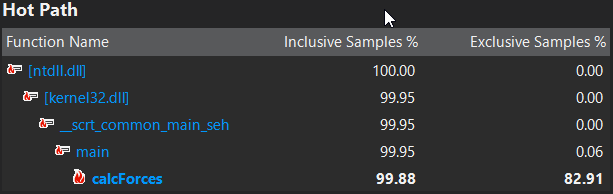
\includegraphics[width=\columnwidth]{IMAGES/hotpath}
		\caption{A image showing the results of running Visual Studio's Performance Profiler, where the "Hot Path" is displayed.}
		\label{figure1}
	\end{figure}
	
	This method, therefore, was the area that was parallelised in attempt to improve performance. However, when there was only 2 bodies the method executed very quickly showing that each individual comparison between bodies required little processing time. The high processing time when there was a large number of bodies was simply that there were so many comparisons to be made. This opened up GPU parallelisation as a potential solution given the large number of lower clock-speed cores.
	
	\section{Methodology}
	
	A systematic approach was undertaken to evaluate the performance of the algorithm and to measure any improvements in performance gained by parallelising the algorithm. The parallelising technologies were chosen based on the results of the initial analysis and on their ability to maximise the performance of the application.
	
	The first step was to run a series of tests on the application to determine likely areas that could be parallelised and which technologies would be suitable, and to provide a baseline that the performance of the different parallel implementations could be compared to. These tests were all done on the same hardware, the relevant specifications of which are shown in table \ref{hardware}. The details of the tests are shown in the testing subsection below.
	
	\begin{table}[!h]
		\renewcommand{\arraystretch}{1.3}
		\caption{Hardware Specifications}
		\label{hardware}
		\centering
		\begin{tabular}{r|l}
			\toprule
			CPU & i7-4790K 4 Core HT @ 4.00GHz\\ \hline
			GPU & NVIDIA GeForce GTX 980 \\ \hline
			RAM & 16.0GB\\ \hline
			OS & Windows 10 Pro 64-bit\\ \bottomrule
		\end{tabular}
	\end{table}
	
	\subsection{Parallelisation Techniques}
	After these benchmarks for the sequential algorithm were recorded, the chosen parallelising techniques were applied to the algorithm and some preliminary simulations were run, each time checking the visualised output of the application. The intention here was twofold; to ensure that the techniques had been implemented correctly, that the parallelised algorithm was still producing the same simulation as the sequential application, and to gain an idea of their relative performance. The techniques used were OpenMP and CUDA, and the parallelisation was only applied to the $calcForces$ method as it took the majority of processing time and in an attempt to reduce accidental speedup to the application beyond simply parallelising the sequential algorithm itself.
	
	\subsubsection{OpenMP}
	OpenMP is an API that supports shared-memory parallel programming and allows some additional manipulations in the scheduling that were used in an attempt to increase performance. The pre-processor argument shown in Listing 1 was used to parallelise the outer forloop, allowing the force calculation algorithm to be run across multiple threads.
	
	\lstinputlisting[caption = The OpenMP parallel for used to parallelise the shown forloop across the number of threads desired.]{./sourceCode/omp.cpp}
	
	OpenMP's parallel for function comes with a \textit{schedule} clause, seen in Listing 1, that was set to static as each iteration of the loop took the same amount of time to process. OpenMP was chosen as a parallel technique as the initial analysis showed that the $calcForces$ method was taking a long time to compute when run sequentially, and parallelising this algorithm so that it could run on multiple threads simultaneously would improve the performance of the application. OpenMP was chosen as it provides this parallelisation simply and effectively across the available CPU cores.
	
	\subsubsection{CUDA}
	CUDA is an API and parallel computing platform created by NVIDIA that allows software to utilise a CUDA-enabled GPU's virtual instruction set and execute the application in parallel using compute kernels. CUDA allows the user to determine the number of \textit{blocks} and \textit{threads per block}, showing in Listing 2, to be used for the kernel method and some testing was done to determine the optimal ratios. Below is an excerpt from the CUDA application.
	
	\lstinputlisting[caption = The $calcForces$ method with CUDA adjustments made and how the kernel method is called within the $main$.]{./sourceCode/cuda.cu}
	
	CUDA was chosen as a notable contrast to OpenMP as it runs on the GPU and would enable a comparison between their respective performance. Further to this, given the results of the initial analysis, executing the $calcForces$ method in parallel on the GPU would provide significant speedup, especially for larger numbers of particles, due to the large number of available cores.
	
	\subsection{Testing}
	The same series of tests that were run on the sequential algorithm in the initial analysis were then undertaken for each implemented parallelisation. These tests were done under the same conditions and on the same hardware to eliminate discrepancies. For the majority of the OpenMP tests, the algorithm was run on the maximum number of threads available. CUDA allowed effective cores in use to be determined as attributes in the kernel method, therefore some initial testing was done on the performance of the application with the number of \textit{threads per block} manipulated.
	
	The testing parameters used to evaluate the performance of the algorithms and the tests themselves are listed below.
	
	For all tests the dependent variable being measured was the amount of time it took for the algorithms to produce the required number of iterations of the simulation. For each change in the independent variables, 100 tests were run and the time it took for the algorithm to produce the necessary values recorded, before the average run times were calculated. 
	
	\begin{enumerate}
		\item CUDA's Threads Per Block
		\begin{itemize}
			\item 	Independent variables: threads per block (from 1 to 32 incremented by powers of 2).
			\item 	Constants: number of simulations (1000), number of bodies (1024).
		\end{itemize}
		\item CUDA and OpenMP Comparisons
		\begin{itemize}
			\item 	Independent variables: number of bodies (from 64 to 4096 incremented by powers of 2)
			\item 	Shared constants: number of simulations (1000).
			\item	CUDA constants: threads per block (8), blocks (number of bodies divided by threads per block).
			\item OpenMP constants: threads (8).
		\end{itemize}
		\item Single Thread Tests
		\begin{itemize}
			\item 	Independent variables: each algorithm (sequential, CUDA, OpenMP).	
			\item 	Constants: number of simulations (1000), number of bodies (512), threads (1).
		\end{itemize}
	\end{enumerate}
	
	\subsection{Evaluation}
	The results of these tests were then collated and compared to the results from the sequential algorithm's testing and used as the basis for the evaluation of their respective performance.
	
	To represent the improved performance, the speedup, $S$, and efficiency, $E$, of the algorithms was calculated using the formula shown in Equation \ref{efficiencyeq} below:
	
	\begin{equation} \label{efficiencyeq} 
		S = \dfrac{T_{serial}}{T_{parallel}}, \qquad E = \dfrac{S}{p}
	\end{equation}
	
	Where $T_{serial}$ and $T_{parallel}$ are the sequential and parallel computational times respectively, and $p$ is the number of processor cores.
	
	\section{Results and Discussion}
	
	\textit{Suitably comprehensive set of results gathered, including investigation of different variables. The results are presented well. Correct charts are used, and these are of a high-standard, including correct scaling. Speedup and efficiency measures provided for all experiments using the correct values.}
	
	The results of the initial \textit{threads per block} test on the CUDA application can be found in \ref{cudathreadtable}.
	The results from the performance testing done on the algorithms can be seen summarised in tables \ref{comptable} and \ref{comptable2} below. As discussed in the initial analysis there is an almost perfect positive correlation between the average time and the increasing samples per pixel and image dimensions for the sequential algorithm, but this also holds true for parallel algorithms. However, the times in which the parallel algorithms produced the data were much lower than the sequential algorithm, even at extreme values (Table \ref{comptable3}).
	
	Table \ref{comptable1} and its accompanying graph (Figure \ref{graph1}) comparing the average time taken for the algorithms to generate the data required to produce a 256x256 image at different numbers of samples per pixel are shown below.
	
	
	\begin{table}[!h]
		\caption{CUDA Performance: Threads Per Block}
		\label{cudathreadtable}
		\centering
		\resizebox{\columnwidth}{!}{%
			\begin{tabular}{cc}
				\toprule
				\multicolumn{2}{c}{Number of Bodies = 1024, Number of Iterations = 1000} \\ \midrule
				\multicolumn{1}{c|}{Threads Per Block} & Average Time / ms \\ \midrule
				\multicolumn{1}{c|}{1} & 3126.17 \\
				\multicolumn{1}{c|}{2} & 1183.69 \\
				\multicolumn{1}{c|}{4} & 1051.98 \\
				\multicolumn{1}{c|}{8} & 1058.97 \\
				\multicolumn{1}{c|}{16} & 1117.77 \\
				\multicolumn{1}{c|}{32} & 1256.76\\ \bottomrule
			\end{tabular}%
		}
	\end{table}
	
	\begin{table}[!h]
		\caption{1000 Iterations N-Body Simulation}
		\label{comptable}
		\centering
		\resizebox{\columnwidth}{!}{%
			\begin{tabular}{cccc}
				\toprule
				\multicolumn{4}{c}{Number of Iterations = 1000} \\ \midrule
				\multicolumn{1}{c|}{Algorithm} & \multicolumn{1}{c}{Sequential} & \multicolumn{1}{c}{OpenMP} & \multicolumn{1}{c}{CUDA} \\ \midrule
				\multicolumn{1}{c|}{Number of Bodies} & \multicolumn{3}{c}{Average Time / ms} \\ \midrule
				\multicolumn{1}{c|}{64} & 20.39 & 15.46 & 105.75 \\
				\multicolumn{1}{c|}{128} & 80.87 & 45.81 & 156.79 \\
				\multicolumn{1}{c|}{256} & 322.96 & 148.66 & 285.48 \\
				\multicolumn{1}{c|}{512} & 1289.07 & 533.66 & 528.34 \\
				\multicolumn{1}{c|}{1024} & 5119.45 & 2007.81 & 1063.36 \\
				\multicolumn{1}{c|}{2048} & 20196.89 & 7820.01 & 2398.78 \\
				\multicolumn{1}{c|}{4096} & 80797.32 & 30628.95 & 6822.16 \\ \bottomrule
			\end{tabular}%
		}
	\end{table}
	
	\begin{figure*}[!h]
		\centering
		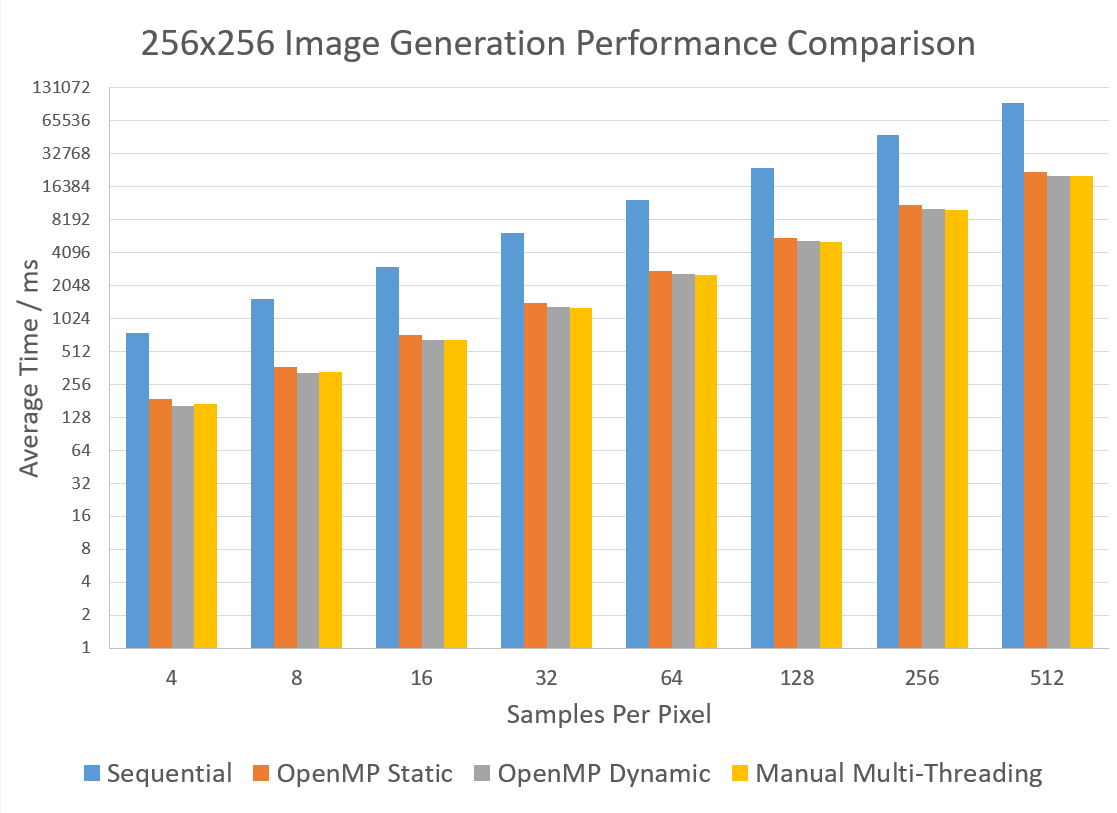
\includegraphics[width=\textwidth]{IMAGES/performancecomparison1}
		\caption{A graph showing the average time it took each algorithm to generate a 256x256 image at different numbers of samples per pixel.}
		\label{graph1}
	\end{figure*}
	
	As the number of samples per pixel were incremented in powers of 2, the data is discrete and the $x$-axis has been displayed using a base-2 logarithmic scale. As a result of this the $y$-axis is also displayed using a base-2 logarithmic scale so that data does not appear skewed. Here we can see that all the parallel algorithms show significant speedup over the sequential algorithm, with the manual multi-threading often being the fastest, if only by a small margin.
	
	The results of the next tests are shown in Table \ref{comptable2}. This table shows the average time it took the algorithms to produce the data for images of varying sizes at 16 samples per pixel. This data is visualised in Figure \ref{graph2} below.

	\begin{figure}[!h]
		\centering
		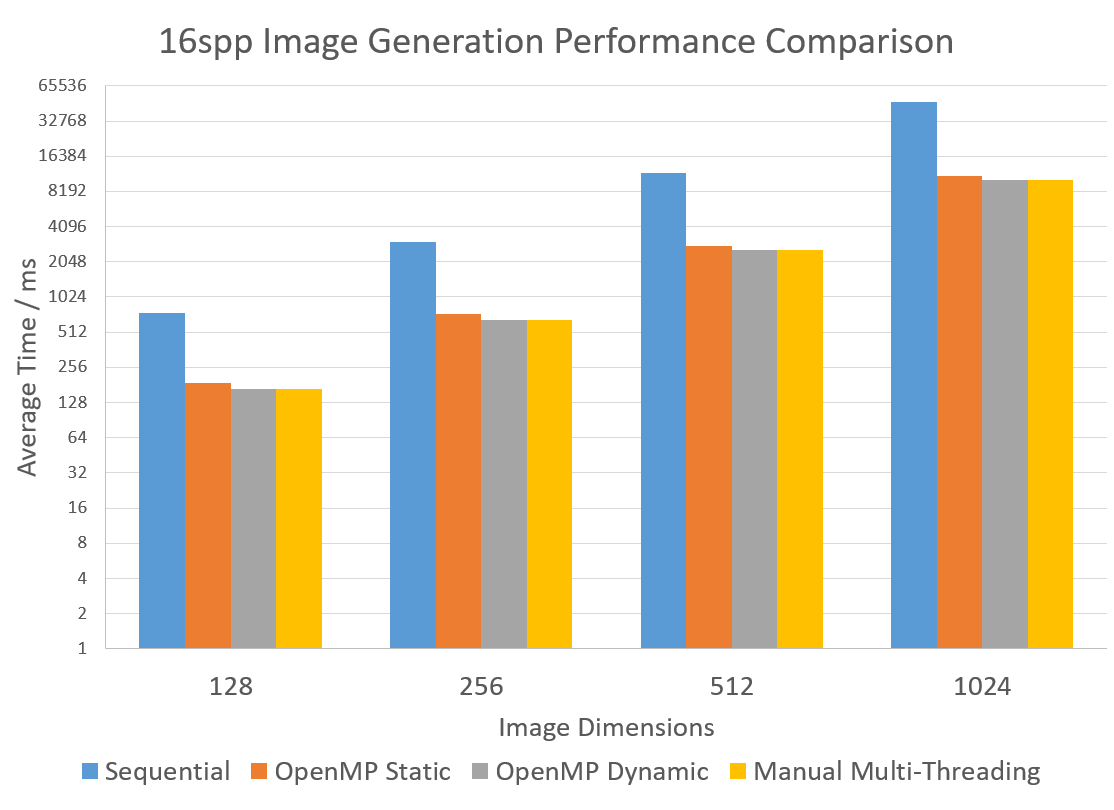
\includegraphics[width=\columnwidth]{IMAGES/performancecomparison2}
		\caption{A graph showing the average time it took each algorithm to generate images of varying dimensions at 16 samples per pixel.}
		\label{graph2}
	\end{figure}

	Once again, the dimensions used for the size of the image were incremented in powers of 2, resulting in a similarly scaled $x$- and $y$-axis, as before. The data from these tests are in line with the previous results. Again it can be seen that the parallel algorithms outperform the sequential algorithm.
	
	There were also a smaller number of tests done at extreme values to compare the algorithm's performances when generating large, high detail images. This is shown in Table \ref{comptable3} below. The data was in agreement with the rest and showed that even at the extreme end the parallelised algorithms generated the images much faster.
	
	By running these averaged times through the formula shown in Equation \ref{efficiencyeq}, the efficiency of these algorithms compared against the sequential algorithm was calculated. The below table (Table \ref{efficiencytable}) shows these efficiencies for the first set of test results.

	\begin{table}[!h]
		\caption{Algorithmic Efficiency Comparison}
		\label{efficiencytable}
		\centering
		\resizebox{\columnwidth}{!}{%
			\begin{tabular}{@{}cccc@{}}
				\toprule
				\multicolumn{4}{c}{Samples Per Pixel = 16} \\ \midrule
				\multicolumn{1}{c|}{Algorithm} & \multicolumn{1}{c}{OMP Static} & \multicolumn{1}{c}{OMP Dynamic} & \multicolumn{1}{c}{Manual} \\ \midrule
				\multicolumn{1}{c|}{Image Dimensions} & \multicolumn{3}{c}{Efficiency} \\ \midrule
				\multicolumn{1}{c|}{128} & 0.997 & 1.125 & 1.108 \\
				\multicolumn{1}{c|}{256} & 1.033 & 1.151 & 1.166 \\
				\multicolumn{1}{c|}{512} & 1.054 & 1.150 & 1.151 \\
				\multicolumn{1}{c|}{1024} & 1.078 & 1.163 & 1.174 \\ \bottomrule
			\end{tabular}%
		}
	\end{table}

	This table shows that some of the algorithms tested had efficiency ratings of more than 1, implying that they ran faster per thread than the sequential algorithm. As stated in the methodology, a few additional tests were done on the parallel algorithms where the number of threads they ran on was controlled. This allowed for a comparison to be made between each algorithm's single threaded performance in order to better contextualise the efficiency ratings of more than 1. Below are two graphs (Figures \ref{graph3} and \ref{graph4}) which show some of the results from these tests.

	\begin{figure}[!h]
		\centering
		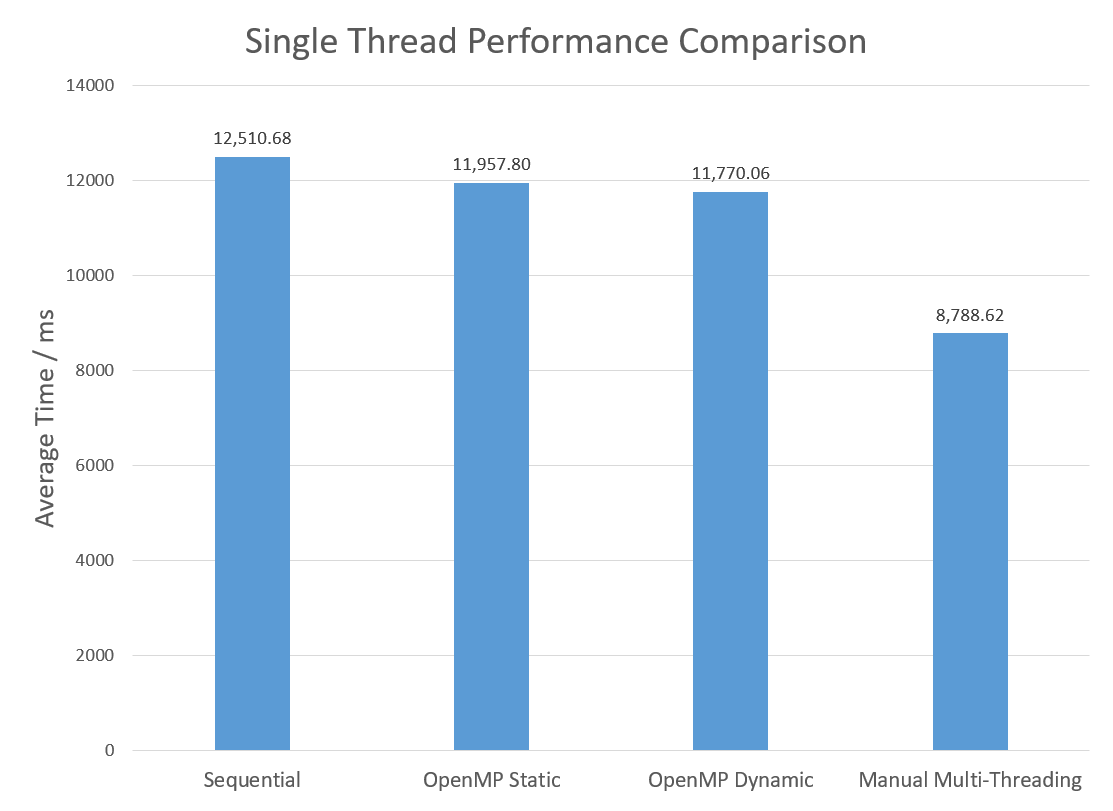
\includegraphics[width=\columnwidth]{IMAGES/singlethreadperformance}
		\caption{A graph showing the average time it took each algorithm to generate a 256x256 image at 16 samples per pixel whilst limited to a single thread.}
		\label{graph3}
	\end{figure}

	Even when ran on a single thread the parallel algorithms generated the required data in less time than the sequential algorithm. In particular, the attempt at manual multi-threading produced significantly faster results. Therefore there were some incidental optimisations of the sequential algorithm when it was parallelised.

	\begin{figure}[!h]
		\centering
		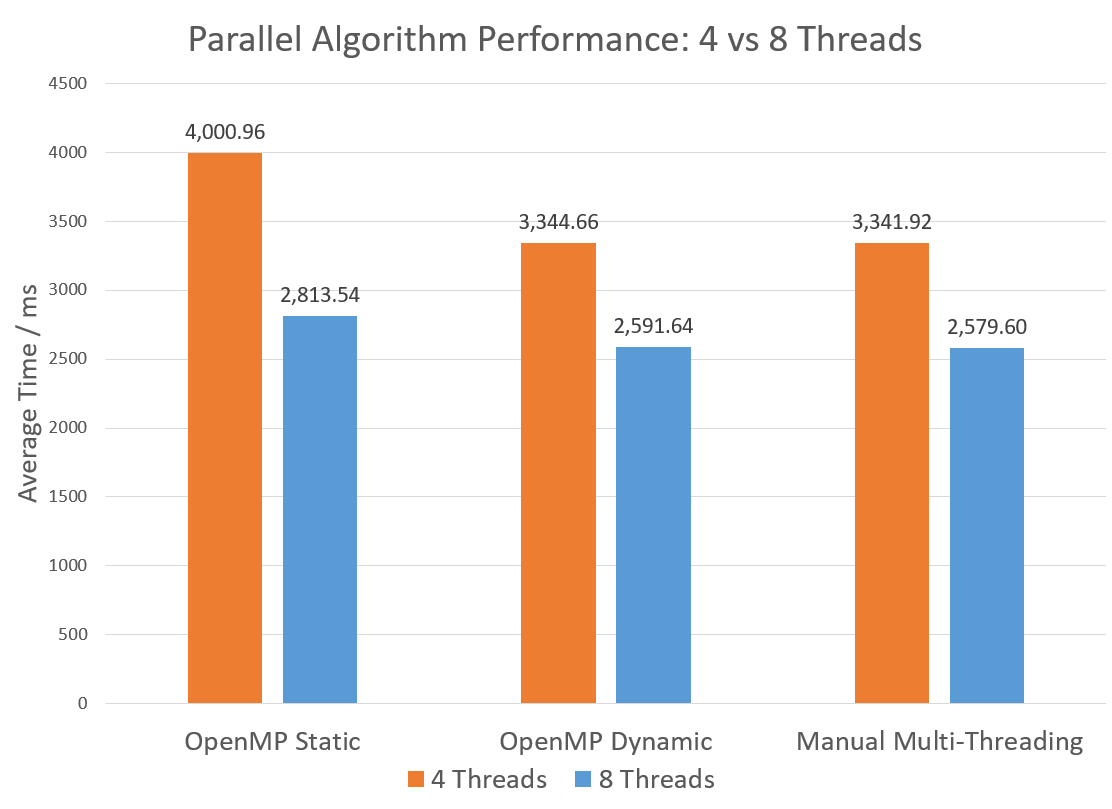
\includegraphics[width=\columnwidth]{IMAGES/threadcomparison}
		\caption{A graph showing the average time it took each algorithm to generate a 256x256 image at 16 samples per pixel on both 4 and 8 threads.}
		\label{graph4}
	\end{figure}

	Further to this, Figure \ref{graph4} shows that there was significant speedup for all the parallelised algorithms when ran on 8 threads instead of 4. The hardware used had 4 cores but allowed for hyper-threading to 8 threads and was potentially a reason for why the efficiencies of more than 1 arose.
	
	\section{Conclusion}
	\subsection{Explanation of Results and Evaluation of Performance}
	Across all the tested algorithms, when either the dimensions of the image or the number of samples per pixel were increased, the time it took to produce the data in the pixel vector used to generate the image would increase with near perfect positive correlation. Furthermore, as shown in Figures \ref{graph1} and \ref{graph2}, independent of whether the image dimensions or the samples per pixels were changed, each of the parallelised algorithms significantly outperformed the sequential algorithm. Compared against each other, OpenMP with static scheduling was always outperformed by both OpenMP with dynamic scheduling	 and the manually multi-threaded algorithm. The manually multi-threading algorithm was generally equal to, or very slightly faster than OpenMP with dynamic scheduling.
	
	Each of the parallelised algorithms had a speedup of 4 or more when compared to the sequential algorithm, and efficiency ratings more than 1. The reasons that the algorithm's efficiency ratings were able to be higher than 1 are likely twofold. Firstly, as shown in Figure \ref{graph3}, the parallelised algorithms were able to generate images quicker than the sequential algorithm even when operating on a single thread. This shows that there were optimisations implemented when parallelising the algorithm, this is especially true for the manually multi-threaded algorithm. Secondly, as shown in Figure \ref{graph4}, there was noticeable speedup from all the algorithms when going from running on 4 threads to running on 8. Given that there were only 4 physical cores and that the equation used to calculate efficiency uses this, a significant proportion of the speedup of the parallelised algorithms is due to the hyper-threading done by the CPU. 
	
	Combined, these two effects make a significant effect on the parallelised algorithm's efficiency ratings. Whilst both parallel algorithms that used OpenMP were only very slightly faster on a single thread than the sequential algorithm, the manually multi-threaded algorithm had a speedup of 1.42 whilst still operating on a single thread. This shows that the performance gained by manually multi-threading the algorithm had much less to do with running the algorithm over multiple threads than the performance gained by the OpenMP parallelised algorithms. The speedup from the hyper-threading, however was more even across the parallelised algorithms.
	
	\subsection{Final Thoughts}
	The provided sequential algorithm originally took a considerable amount of time to produce large images of quality. The attempts at parallelising the algorithm were largely successful. They all performed significantly faster than the sequential algorithm and made the time to generate large images of high detail more manageable. However, whilst running on multiple threads did provide speedup, an important part of the increased performance of the algorithms was due to external optimisations. The attempt at manually multi-threading the algorithm benefited the most from this and as such ended up outperforming both versions of parallelisation using OpenMP. In terms of increased performance purely due to running the algorithm across multiple threads the algorithm that was dynamically scheduled using OpenMP was the top performer.
	
	\bibliographystyle{IEEEtran}
	\bibliography{bibliography}
	
	\newpage
	\onecolumn
	\appendices
	\section{raytracer.cpp}
	\lstinputlisting[caption = The source code for the raytracer.cpp including all the added parallelisation techniques.]{./sourceCode/raytracer.cpp}
	
\end{document}